
\documentclass[11pt]{article}

%\usepackage[T1]{fontenc}\usepackage{ae,aecompl}
\usepackage[T1]{fontenc}\usepackage{pslatex}

    \usepackage[breakable]{tcolorbox}
    
    \usepackage{parskip} % Stop auto-indenting (to mimic markdown behaviour)
    
    \usepackage{iftex}
    \ifPDFTeX
    	\usepackage[T1]{fontenc}
    	\usepackage{mathpazo}
    \else
    	\usepackage{fontspec}
    \fi

    % Basic figure setup, for now with no caption control since it's done
    % automatically by Pandoc (which extracts ![](path) syntax from Markdown).
    \usepackage{graphicx}
    % Maintain compatibility with old templates. Remove in nbconvert 6.0
    \let\Oldincludegraphics\includegraphics
    % Ensure that by default, figures have no caption (until we provide a
    % proper Figure object with a Caption API and a way to capture that
    % in the conversion process - todo).
    \usepackage{caption}
    \DeclareCaptionFormat{nocaption}{}
    \captionsetup{format=nocaption,aboveskip=0pt,belowskip=0pt}

    \usepackage{float}
    \floatplacement{figure}{H} % forces figures to be placed at the correct location
    \usepackage{xcolor} % Allow colors to be defined
    \usepackage{enumerate} % Needed for markdown enumerations to work
    \usepackage{geometry} % Used to adjust the document margins
    \usepackage{amsmath} % Equations
    \usepackage{amssymb} % Equations
    \usepackage{textcomp} % defines textquotesingle
    % Hack from http://tex.stackexchange.com/a/47451/13684:
    \AtBeginDocument{%
        \def\PYZsq{\textquotesingle}% Upright quotes in Pygmentized code
    }
    \usepackage{upquote} % Upright quotes for verbatim code
    \usepackage{eurosym} % defines \euro
    \usepackage[mathletters]{ucs} % Extended unicode (utf-8) support
    \usepackage{fancyvrb} % verbatim replacement that allows latex
    \usepackage{grffile} % extends the file name processing of package graphics 
                         % to support a larger range
    \makeatletter % fix for old versions of grffile with XeLaTeX
    \@ifpackagelater{grffile}{2019/11/01}
    {
      % Do nothing on new versions
    }
    {
      \def\Gread@@xetex#1{%
        \IfFileExists{"\Gin@base".bb}%
        {\Gread@eps{\Gin@base.bb}}%
        {\Gread@@xetex@aux#1}%
      }
    }
    \makeatother
    \usepackage[Export]{adjustbox} % Used to constrain images to a maximum size
    \adjustboxset{max size={0.9\linewidth}{0.9\paperheight}}

    % The hyperref package gives us a pdf with properly built
    % internal navigation ('pdf bookmarks' for the table of contents,
    % internal cross-reference links, web links for URLs, etc.)
    \usepackage{hyperref}
    % The default LaTeX title has an obnoxious amount of whitespace. By default,
    % titling removes some of it. It also provides customization options.
    \usepackage{titling}
    \usepackage{longtable} % longtable support required by pandoc >1.10
    \usepackage{booktabs}  % table support for pandoc > 1.12.2
    \usepackage[inline]{enumitem} % IRkernel/repr support (it uses the enumerate* environment)
    \usepackage[normalem]{ulem} % ulem is needed to support strikethroughs (\sout)
                                % normalem makes italics be italics, not underlines
    \usepackage{mathrsfs}
    

    
    % Colors for the hyperref package
    \definecolor{urlcolor}{rgb}{0,.145,.698}
    \definecolor{linkcolor}{rgb}{.71,0.21,0.01}
    \definecolor{citecolor}{rgb}{.12,.54,.11}

    % ANSI colors
    \definecolor{ansi-black}{HTML}{3E424D}
    \definecolor{ansi-black-intense}{HTML}{282C36}
    \definecolor{ansi-red}{HTML}{E75C58}
    \definecolor{ansi-red-intense}{HTML}{B22B31}
    \definecolor{ansi-green}{HTML}{00A250}
    \definecolor{ansi-green-intense}{HTML}{007427}
    \definecolor{ansi-yellow}{HTML}{DDB62B}
    \definecolor{ansi-yellow-intense}{HTML}{B27D12}
    \definecolor{ansi-blue}{HTML}{208FFB}
    \definecolor{ansi-blue-intense}{HTML}{0065CA}
    \definecolor{ansi-magenta}{HTML}{D160C4}
    \definecolor{ansi-magenta-intense}{HTML}{A03196}
    \definecolor{ansi-cyan}{HTML}{60C6C8}
    \definecolor{ansi-cyan-intense}{HTML}{258F8F}
    \definecolor{ansi-white}{HTML}{C5C1B4}
    \definecolor{ansi-white-intense}{HTML}{A1A6B2}
    \definecolor{ansi-default-inverse-fg}{HTML}{FFFFFF}
    \definecolor{ansi-default-inverse-bg}{HTML}{000000}

    % common color for the border for error outputs.
    \definecolor{outerrorbackground}{HTML}{FFDFDF}

    % commands and environments needed by pandoc snippets
    % extracted from the output of `pandoc -s`
    \providecommand{\tightlist}{%
      \setlength{\itemsep}{0pt}\setlength{\parskip}{0pt}}
    \DefineVerbatimEnvironment{Highlighting}{Verbatim}{commandchars=\\\{\}}
    % Add ',fontsize=\small' for more characters per line
    \newenvironment{Shaded}{}{}
    \newcommand{\KeywordTok}[1]{\textcolor[rgb]{0.00,0.44,0.13}{\textbf{{#1}}}}
    \newcommand{\DataTypeTok}[1]{\textcolor[rgb]{0.56,0.13,0.00}{{#1}}}
    \newcommand{\DecValTok}[1]{\textcolor[rgb]{0.25,0.63,0.44}{{#1}}}
    \newcommand{\BaseNTok}[1]{\textcolor[rgb]{0.25,0.63,0.44}{{#1}}}
    \newcommand{\FloatTok}[1]{\textcolor[rgb]{0.25,0.63,0.44}{{#1}}}
    \newcommand{\CharTok}[1]{\textcolor[rgb]{0.25,0.44,0.63}{{#1}}}
    \newcommand{\StringTok}[1]{\textcolor[rgb]{0.25,0.44,0.63}{{#1}}}
    \newcommand{\CommentTok}[1]{\textcolor[rgb]{0.38,0.63,0.69}{\textit{{#1}}}}
    \newcommand{\OtherTok}[1]{\textcolor[rgb]{0.00,0.44,0.13}{{#1}}}
    \newcommand{\AlertTok}[1]{\textcolor[rgb]{1.00,0.00,0.00}{\textbf{{#1}}}}
    \newcommand{\FunctionTok}[1]{\textcolor[rgb]{0.02,0.16,0.49}{{#1}}}
    \newcommand{\RegionMarkerTok}[1]{{#1}}
    \newcommand{\ErrorTok}[1]{\textcolor[rgb]{1.00,0.00,0.00}{\textbf{{#1}}}}
    \newcommand{\NormalTok}[1]{{#1}}
    
    % Additional commands for more recent versions of Pandoc
    \newcommand{\ConstantTok}[1]{\textcolor[rgb]{0.53,0.00,0.00}{{#1}}}
    \newcommand{\SpecialCharTok}[1]{\textcolor[rgb]{0.25,0.44,0.63}{{#1}}}
    \newcommand{\VerbatimStringTok}[1]{\textcolor[rgb]{0.25,0.44,0.63}{{#1}}}
    \newcommand{\SpecialStringTok}[1]{\textcolor[rgb]{0.73,0.40,0.53}{{#1}}}
    \newcommand{\ImportTok}[1]{{#1}}
    \newcommand{\DocumentationTok}[1]{\textcolor[rgb]{0.73,0.13,0.13}{\textit{{#1}}}}
    \newcommand{\AnnotationTok}[1]{\textcolor[rgb]{0.38,0.63,0.69}{\textbf{\textit{{#1}}}}}
    \newcommand{\CommentVarTok}[1]{\textcolor[rgb]{0.38,0.63,0.69}{\textbf{\textit{{#1}}}}}
    \newcommand{\VariableTok}[1]{\textcolor[rgb]{0.10,0.09,0.49}{{#1}}}
    \newcommand{\ControlFlowTok}[1]{\textcolor[rgb]{0.00,0.44,0.13}{\textbf{{#1}}}}
    \newcommand{\OperatorTok}[1]{\textcolor[rgb]{0.40,0.40,0.40}{{#1}}}
    \newcommand{\BuiltInTok}[1]{{#1}}
    \newcommand{\ExtensionTok}[1]{{#1}}
    \newcommand{\PreprocessorTok}[1]{\textcolor[rgb]{0.74,0.48,0.00}{{#1}}}
    \newcommand{\AttributeTok}[1]{\textcolor[rgb]{0.49,0.56,0.16}{{#1}}}
    \newcommand{\InformationTok}[1]{\textcolor[rgb]{0.38,0.63,0.69}{\textbf{\textit{{#1}}}}}
    \newcommand{\WarningTok}[1]{\textcolor[rgb]{0.38,0.63,0.69}{\textbf{\textit{{#1}}}}}
    
    
    % Define a nice break command that doesn't care if a line doesn't already
    % exist.
    \def\br{\hspace*{\fill} \\* }
    % Math Jax compatibility definitions
    \def\gt{>}
    \def\lt{<}
    \let\Oldtex\TeX
    \let\Oldlatex\LaTeX
    \renewcommand{\TeX}{\textrm{\Oldtex}}
    \renewcommand{\LaTeX}{\textrm{\Oldlatex}}
    % Document parameters
    % Document title
  
    
\title{GitTutorial}

\author{Edgardo Bonzi}
    
    
% Pygments definitions
\makeatletter
\def\PY@reset{\let\PY@it=\relax \let\PY@bf=\relax%
    \let\PY@ul=\relax \let\PY@tc=\relax%
    \let\PY@bc=\relax \let\PY@ff=\relax}
\def\PY@tok#1{\csname PY@tok@#1\endcsname}
\def\PY@toks#1+{\ifx\relax#1\empty\else%
    \PY@tok{#1}\expandafter\PY@toks\fi}
\def\PY@do#1{\PY@bc{\PY@tc{\PY@ul{%
    \PY@it{\PY@bf{\PY@ff{#1}}}}}}}
\def\PY#1#2{\PY@reset\PY@toks#1+\relax+\PY@do{#2}}

\@namedef{PY@tok@w}{\def\PY@tc##1{\textcolor[rgb]{0.73,0.73,0.73}{##1}}}
\@namedef{PY@tok@c}{\let\PY@it=\textit\def\PY@tc##1{\textcolor[rgb]{0.25,0.50,0.50}{##1}}}
\@namedef{PY@tok@cp}{\def\PY@tc##1{\textcolor[rgb]{0.74,0.48,0.00}{##1}}}
\@namedef{PY@tok@k}{\let\PY@bf=\textbf\def\PY@tc##1{\textcolor[rgb]{0.00,0.50,0.00}{##1}}}
\@namedef{PY@tok@kp}{\def\PY@tc##1{\textcolor[rgb]{0.00,0.50,0.00}{##1}}}
\@namedef{PY@tok@kt}{\def\PY@tc##1{\textcolor[rgb]{0.69,0.00,0.25}{##1}}}
\@namedef{PY@tok@o}{\def\PY@tc##1{\textcolor[rgb]{0.40,0.40,0.40}{##1}}}
\@namedef{PY@tok@ow}{\let\PY@bf=\textbf\def\PY@tc##1{\textcolor[rgb]{0.67,0.13,1.00}{##1}}}
\@namedef{PY@tok@nb}{\def\PY@tc##1{\textcolor[rgb]{0.00,0.50,0.00}{##1}}}
\@namedef{PY@tok@nf}{\def\PY@tc##1{\textcolor[rgb]{0.00,0.00,1.00}{##1}}}
\@namedef{PY@tok@nc}{\let\PY@bf=\textbf\def\PY@tc##1{\textcolor[rgb]{0.00,0.00,1.00}{##1}}}
\@namedef{PY@tok@nn}{\let\PY@bf=\textbf\def\PY@tc##1{\textcolor[rgb]{0.00,0.00,1.00}{##1}}}
\@namedef{PY@tok@ne}{\let\PY@bf=\textbf\def\PY@tc##1{\textcolor[rgb]{0.82,0.25,0.23}{##1}}}
\@namedef{PY@tok@nv}{\def\PY@tc##1{\textcolor[rgb]{0.10,0.09,0.49}{##1}}}
\@namedef{PY@tok@no}{\def\PY@tc##1{\textcolor[rgb]{0.53,0.00,0.00}{##1}}}
\@namedef{PY@tok@nl}{\def\PY@tc##1{\textcolor[rgb]{0.63,0.63,0.00}{##1}}}
\@namedef{PY@tok@ni}{\let\PY@bf=\textbf\def\PY@tc##1{\textcolor[rgb]{0.60,0.60,0.60}{##1}}}
\@namedef{PY@tok@na}{\def\PY@tc##1{\textcolor[rgb]{0.49,0.56,0.16}{##1}}}
\@namedef{PY@tok@nt}{\let\PY@bf=\textbf\def\PY@tc##1{\textcolor[rgb]{0.00,0.50,0.00}{##1}}}
\@namedef{PY@tok@nd}{\def\PY@tc##1{\textcolor[rgb]{0.67,0.13,1.00}{##1}}}
\@namedef{PY@tok@s}{\def\PY@tc##1{\textcolor[rgb]{0.73,0.13,0.13}{##1}}}
\@namedef{PY@tok@sd}{\let\PY@it=\textit\def\PY@tc##1{\textcolor[rgb]{0.73,0.13,0.13}{##1}}}
\@namedef{PY@tok@si}{\let\PY@bf=\textbf\def\PY@tc##1{\textcolor[rgb]{0.73,0.40,0.53}{##1}}}
\@namedef{PY@tok@se}{\let\PY@bf=\textbf\def\PY@tc##1{\textcolor[rgb]{0.73,0.40,0.13}{##1}}}
\@namedef{PY@tok@sr}{\def\PY@tc##1{\textcolor[rgb]{0.73,0.40,0.53}{##1}}}
\@namedef{PY@tok@ss}{\def\PY@tc##1{\textcolor[rgb]{0.10,0.09,0.49}{##1}}}
\@namedef{PY@tok@sx}{\def\PY@tc##1{\textcolor[rgb]{0.00,0.50,0.00}{##1}}}
\@namedef{PY@tok@m}{\def\PY@tc##1{\textcolor[rgb]{0.40,0.40,0.40}{##1}}}
\@namedef{PY@tok@gh}{\let\PY@bf=\textbf\def\PY@tc##1{\textcolor[rgb]{0.00,0.00,0.50}{##1}}}
\@namedef{PY@tok@gu}{\let\PY@bf=\textbf\def\PY@tc##1{\textcolor[rgb]{0.50,0.00,0.50}{##1}}}
\@namedef{PY@tok@gd}{\def\PY@tc##1{\textcolor[rgb]{0.63,0.00,0.00}{##1}}}
\@namedef{PY@tok@gi}{\def\PY@tc##1{\textcolor[rgb]{0.00,0.63,0.00}{##1}}}
\@namedef{PY@tok@gr}{\def\PY@tc##1{\textcolor[rgb]{1.00,0.00,0.00}{##1}}}
\@namedef{PY@tok@ge}{\let\PY@it=\textit}
\@namedef{PY@tok@gs}{\let\PY@bf=\textbf}
\@namedef{PY@tok@gp}{\let\PY@bf=\textbf\def\PY@tc##1{\textcolor[rgb]{0.00,0.00,0.50}{##1}}}
\@namedef{PY@tok@go}{\def\PY@tc##1{\textcolor[rgb]{0.53,0.53,0.53}{##1}}}
\@namedef{PY@tok@gt}{\def\PY@tc##1{\textcolor[rgb]{0.00,0.27,0.87}{##1}}}
\@namedef{PY@tok@err}{\def\PY@bc##1{{\setlength{\fboxsep}{\string -\fboxrule}\fcolorbox[rgb]{1.00,0.00,0.00}{1,1,1}{\strut ##1}}}}
\@namedef{PY@tok@kc}{\let\PY@bf=\textbf\def\PY@tc##1{\textcolor[rgb]{0.00,0.50,0.00}{##1}}}
\@namedef{PY@tok@kd}{\let\PY@bf=\textbf\def\PY@tc##1{\textcolor[rgb]{0.00,0.50,0.00}{##1}}}
\@namedef{PY@tok@kn}{\let\PY@bf=\textbf\def\PY@tc##1{\textcolor[rgb]{0.00,0.50,0.00}{##1}}}
\@namedef{PY@tok@kr}{\let\PY@bf=\textbf\def\PY@tc##1{\textcolor[rgb]{0.00,0.50,0.00}{##1}}}
\@namedef{PY@tok@bp}{\def\PY@tc##1{\textcolor[rgb]{0.00,0.50,0.00}{##1}}}
\@namedef{PY@tok@fm}{\def\PY@tc##1{\textcolor[rgb]{0.00,0.00,1.00}{##1}}}
\@namedef{PY@tok@vc}{\def\PY@tc##1{\textcolor[rgb]{0.10,0.09,0.49}{##1}}}
\@namedef{PY@tok@vg}{\def\PY@tc##1{\textcolor[rgb]{0.10,0.09,0.49}{##1}}}
\@namedef{PY@tok@vi}{\def\PY@tc##1{\textcolor[rgb]{0.10,0.09,0.49}{##1}}}
\@namedef{PY@tok@vm}{\def\PY@tc##1{\textcolor[rgb]{0.10,0.09,0.49}{##1}}}
\@namedef{PY@tok@sa}{\def\PY@tc##1{\textcolor[rgb]{0.73,0.13,0.13}{##1}}}
\@namedef{PY@tok@sb}{\def\PY@tc##1{\textcolor[rgb]{0.73,0.13,0.13}{##1}}}
\@namedef{PY@tok@sc}{\def\PY@tc##1{\textcolor[rgb]{0.73,0.13,0.13}{##1}}}
\@namedef{PY@tok@dl}{\def\PY@tc##1{\textcolor[rgb]{0.73,0.13,0.13}{##1}}}
\@namedef{PY@tok@s2}{\def\PY@tc##1{\textcolor[rgb]{0.73,0.13,0.13}{##1}}}
\@namedef{PY@tok@sh}{\def\PY@tc##1{\textcolor[rgb]{0.73,0.13,0.13}{##1}}}
\@namedef{PY@tok@s1}{\def\PY@tc##1{\textcolor[rgb]{0.73,0.13,0.13}{##1}}}
\@namedef{PY@tok@mb}{\def\PY@tc##1{\textcolor[rgb]{0.40,0.40,0.40}{##1}}}
\@namedef{PY@tok@mf}{\def\PY@tc##1{\textcolor[rgb]{0.40,0.40,0.40}{##1}}}
\@namedef{PY@tok@mh}{\def\PY@tc##1{\textcolor[rgb]{0.40,0.40,0.40}{##1}}}
\@namedef{PY@tok@mi}{\def\PY@tc##1{\textcolor[rgb]{0.40,0.40,0.40}{##1}}}
\@namedef{PY@tok@il}{\def\PY@tc##1{\textcolor[rgb]{0.40,0.40,0.40}{##1}}}
\@namedef{PY@tok@mo}{\def\PY@tc##1{\textcolor[rgb]{0.40,0.40,0.40}{##1}}}
\@namedef{PY@tok@ch}{\let\PY@it=\textit\def\PY@tc##1{\textcolor[rgb]{0.25,0.50,0.50}{##1}}}
\@namedef{PY@tok@cm}{\let\PY@it=\textit\def\PY@tc##1{\textcolor[rgb]{0.25,0.50,0.50}{##1}}}
\@namedef{PY@tok@cpf}{\let\PY@it=\textit\def\PY@tc##1{\textcolor[rgb]{0.25,0.50,0.50}{##1}}}
\@namedef{PY@tok@c1}{\let\PY@it=\textit\def\PY@tc##1{\textcolor[rgb]{0.25,0.50,0.50}{##1}}}
\@namedef{PY@tok@cs}{\let\PY@it=\textit\def\PY@tc##1{\textcolor[rgb]{0.25,0.50,0.50}{##1}}}

\def\PYZbs{\char`\\}
\def\PYZus{\char`\_}
\def\PYZob{\char`\{}
\def\PYZcb{\char`\}}
\def\PYZca{\char`\^}
\def\PYZam{\char`\&}
\def\PYZlt{\char`\<}
\def\PYZgt{\char`\>}
\def\PYZsh{\char`\#}
\def\PYZpc{\char`\%}
\def\PYZdl{\char`\$}
\def\PYZhy{\char`\-}
\def\PYZsq{\char`\'}
\def\PYZdq{\char`\"}
\def\PYZti{\char`\~}
% for compatibility with earlier versions
\def\PYZat{@}
\def\PYZlb{[}
\def\PYZrb{]}
\makeatother


    % For linebreaks inside Verbatim environment from package fancyvrb. 
    \makeatletter
        \newbox\Wrappedcontinuationbox 
        \newbox\Wrappedvisiblespacebox 
        \newcommand*\Wrappedvisiblespace {\textcolor{red}{\textvisiblespace}} 
        \newcommand*\Wrappedcontinuationsymbol {\textcolor{red}{\llap{\tiny$\m@th\hookrightarrow$}}} 
        \newcommand*\Wrappedcontinuationindent {3ex } 
        \newcommand*\Wrappedafterbreak {\kern\Wrappedcontinuationindent\copy\Wrappedcontinuationbox} 
        % Take advantage of the already applied Pygments mark-up to insert 
        % potential linebreaks for TeX processing. 
        %        {, <, #, %, $, ' and ": go to next line. 
        %        _, }, ^, &, >, - and ~: stay at end of broken line. 
        % Use of \textquotesingle for straight quote. 
        \newcommand*\Wrappedbreaksatspecials {% 
            \def\PYGZus{\discretionary{\char`\_}{\Wrappedafterbreak}{\char`\_}}% 
            \def\PYGZob{\discretionary{}{\Wrappedafterbreak\char`\{}{\char`\{}}% 
            \def\PYGZcb{\discretionary{\char`\}}{\Wrappedafterbreak}{\char`\}}}% 
            \def\PYGZca{\discretionary{\char`\^}{\Wrappedafterbreak}{\char`\^}}% 
            \def\PYGZam{\discretionary{\char`\&}{\Wrappedafterbreak}{\char`\&}}% 
            \def\PYGZlt{\discretionary{}{\Wrappedafterbreak\char`\<}{\char`\<}}% 
            \def\PYGZgt{\discretionary{\char`\>}{\Wrappedafterbreak}{\char`\>}}% 
            \def\PYGZsh{\discretionary{}{\Wrappedafterbreak\char`\#}{\char`\#}}% 
            \def\PYGZpc{\discretionary{}{\Wrappedafterbreak\char`\%}{\char`\%}}% 
            \def\PYGZdl{\discretionary{}{\Wrappedafterbreak\char`\$}{\char`\$}}% 
            \def\PYGZhy{\discretionary{\char`\-}{\Wrappedafterbreak}{\char`\-}}% 
            \def\PYGZsq{\discretionary{}{\Wrappedafterbreak\textquotesingle}{\textquotesingle}}% 
            \def\PYGZdq{\discretionary{}{\Wrappedafterbreak\char`\"}{\char`\"}}% 
            \def\PYGZti{\discretionary{\char`\~}{\Wrappedafterbreak}{\char`\~}}% 
        } 
        % Some characters . , ; ? ! / are not pygmentized. 
        % This macro makes them "active" and they will insert potential linebreaks 
        \newcommand*\Wrappedbreaksatpunct {% 
            \lccode`\~`\.\lowercase{\def~}{\discretionary{\hbox{\char`\.}}{\Wrappedafterbreak}{\hbox{\char`\.}}}% 
            \lccode`\~`\,\lowercase{\def~}{\discretionary{\hbox{\char`\,}}{\Wrappedafterbreak}{\hbox{\char`\,}}}% 
            \lccode`\~`\;\lowercase{\def~}{\discretionary{\hbox{\char`\;}}{\Wrappedafterbreak}{\hbox{\char`\;}}}% 
            \lccode`\~`\:\lowercase{\def~}{\discretionary{\hbox{\char`\:}}{\Wrappedafterbreak}{\hbox{\char`\:}}}% 
            \lccode`\~`\?\lowercase{\def~}{\discretionary{\hbox{\char`\?}}{\Wrappedafterbreak}{\hbox{\char`\?}}}% 
            \lccode`\~`\!\lowercase{\def~}{\discretionary{\hbox{\char`\!}}{\Wrappedafterbreak}{\hbox{\char`\!}}}% 
            \lccode`\~`\/\lowercase{\def~}{\discretionary{\hbox{\char`\/}}{\Wrappedafterbreak}{\hbox{\char`\/}}}% 
            \catcode`\.\active
            \catcode`\,\active 
            \catcode`\;\active
            \catcode`\:\active
            \catcode`\?\active
            \catcode`\!\active
            \catcode`\/\active 
            \lccode`\~`\~ 	
        }
    \makeatother

    \let\OriginalVerbatim=\Verbatim
    \makeatletter
    \renewcommand{\Verbatim}[1][1]{%
        %\parskip\z@skip
        \sbox\Wrappedcontinuationbox {\Wrappedcontinuationsymbol}%
        \sbox\Wrappedvisiblespacebox {\FV@SetupFont\Wrappedvisiblespace}%
        \def\FancyVerbFormatLine ##1{\hsize\linewidth
            \vtop{\raggedright\hyphenpenalty\z@\exhyphenpenalty\z@
                \doublehyphendemerits\z@\finalhyphendemerits\z@
                \strut ##1\strut}%
        }%
        % If the linebreak is at a space, the latter will be displayed as visible
        % space at end of first line, and a continuation symbol starts next line.
        % Stretch/shrink are however usually zero for typewriter font.
        \def\FV@Space {%
            \nobreak\hskip\z@ plus\fontdimen3\font minus\fontdimen4\font
            \discretionary{\copy\Wrappedvisiblespacebox}{\Wrappedafterbreak}
            {\kern\fontdimen2\font}%
        }%
        
        % Allow breaks at special characters using \PYG... macros.
        \Wrappedbreaksatspecials
        % Breaks at punctuation characters . , ; ? ! and / need catcode=\active 	
        \OriginalVerbatim[#1,codes*=\Wrappedbreaksatpunct]%
    }
    \makeatother

    % Exact colors from NB
    \definecolor{incolor}{HTML}{303F9F}
    \definecolor{outcolor}{HTML}{D84315}
    \definecolor{cellborder}{HTML}{CFCFCF}
    \definecolor{cellbackground}{HTML}{F7F7F7}
    
    % prompt
    \makeatletter
    \newcommand{\boxspacing}{\kern\kvtcb@left@rule\kern\kvtcb@boxsep}
    \makeatother
    \newcommand{\prompt}[4]{
        {\ttfamily\llap{{\color{#2}[#3]:\hspace{3pt}#4}}\vspace{-\baselineskip}}
    }
    

    
    % Prevent overflowing lines due to hard-to-break entities
    \sloppy 
    % Setup hyperref package
    \hypersetup{
      breaklinks=true,  % so long urls are correctly broken across lines
      colorlinks=true,
      urlcolor=urlcolor,
      linkcolor=linkcolor,
      citecolor=citecolor,
      }
    % Slightly bigger margins than the latex defaults
    
    \geometry{verbose,tmargin=1in,bmargin=1in,lmargin=1in,rmargin=1in}
    
    

\begin{document}
    
    \maketitle
    
    

    
    \hypertarget{git-para-principiantes}{%
\section{Git para principiantes}\label{git-para-principiantes}}

    Este notebooks está inspirado en:\\
https://www.ionos.es/digitalguide/paginas-web/desarrollo-web/tutorial-de-git/\\
https://git-scm.com/book/en/v2/Getting-Started-About-Version-Control

    \hypertarget{git-tutorial-buxe1sico-del-sistema-de-control-de-versiones}{%
\subsection{\texorpdfstring{Git: tutorial básico del \textbf{S}istema de
\textbf{C}ontrol de
\textbf{V}ersiones}{Git: tutorial básico del Sistema de Control de Versiones}}\label{git-tutorial-buxe1sico-del-sistema-de-control-de-versiones}}

\textbf{V}ersion \textbf{C}ontrol \textbf{S}ystem (VCS)

    No solo las empresas desarrollan proyectos de software de forma
colaborativa: también en el sector del código abierto, varios cientos o
incluso miles de voluntarios y colaboradores pueden participar en la
creación, el mantenimiento, la optimización o la edición de un programa,
dependiendo del tamaño del proyecto. Sería prácticamente imposible
llevar a cabo estas tareas sin un buen sistemapara registrar y controlar
los numerosos cambios realizados por todos los desarrolladores.

Una de las soluciones más populares en este sentido es Git, un programa
de licencia libre que puedes aprender a manejar rápidamente y utilizar
de forma totalmente gratuita. En nuestro tutorial, te enseñamos todos
los conceptos básicos para que seas capaz de dar tus primeros pasos con
este sistema de control de versiones.

    \hypertarget{quuxe9-es-git}{%
\subsection{¿Qué es Git?}\label{quuxe9-es-git}}

Git es un sistema de control de versiones (VCS) desarrollado en 2005 por
Linus Thorvalds, el creador de Linux, y publicado bajo la licencia de
software libre GPLv2 de GNU.

La particularidad de esta herramienta es que, aunque guarda un
repositorio central para cada proyecto, todos los participantes
descargan una copia local del mismo en su propio dispositivo.

Cada una de estas copias constituye una copia completa de todo el
contenido del repositorio, por lo que no es necesario estar conectado a
la red para trabajar. Además, estos archivos sirven como copia de
seguridad en caso de que el repositorio principal falle o resulte
dañado. Los cambios en los archivos pueden intercambiarse con todos los
demás participantes del proyecto en cualquier momento y, si corresponde,
añadirse al repositorio. Consejo

\begin{quote}
Una de las alternativas más conocidas a \textbf{Git} es
\textbf{Subversion}, una herramienta también de código abierto y más
conocida como SVN, que se basa en un sistema de gestión central,
contrariamente a Git.
\end{quote}

    \hypertarget{cuxf3mo-instalar-git-en-el-dispositivo}{%
\subsection{Cómo instalar Git en el
dispositivo}\label{cuxf3mo-instalar-git-en-el-dispositivo}}

https://git-scm.com/download/linux

Si quieres empezar a utilizar Git como programa de control de versiones,
en primer lugar, debes familiarizarte con el propio software y su
interfaz de usuario.\\
Git está disponible para Windows, Unix/Linux y macOS, con diferentes
versiones que presentan pequeñas diferencias de uso.\\
Después de llevar a cabo la instalación estándar correspondiente, puedes
controlar el programa con el símbolo del sistema o una interfaz gráfica
de usuario en cualquiera de los sistemas operativos. Nota

\begin{quote}
Para poder utilizar los comandos explicados en este tutorial de Git, los
usuarios de Windows deben ejecutarlo a través de Git Bash, un shell de
estilo Unix que emula la línea de comandos de Git y está incluido en el
paquete de instalación. Si lo prefieres, también es posible controlar el
software con el símbolo del sistema o la terminal de Windows, aunque
debes tener en cuenta que la estructura de los parámetros de los
comandos difiere (por ejemplo, se emplean signos de ídem en lugar de
comillas).
\end{quote}

\hypertarget{descargar-para-linuxubuntu}{%
\subsubsection{Descargar para
Linux/Ubuntu}\label{descargar-para-linuxubuntu}}

Es más fácil instalar Git en Linux utilizando el administrador de
paquetes preferido de su distribución de Linux.\\
Si prefiere compilar desde el código fuente, puede encontrar tarballs en
kernel.org. La última versión es la 2.35.1. Debian/Ubuntu

Para obtener la última versión estable para su lanzamiento de
Debian/Ubuntu

\begin{quote}
{[}\textasciitilde{}{]} \$ \textbf{sudo apt update}
\end{quote}

\begin{quote}
{[}\textasciitilde{}{]} \$ \textbf{apt-get install git}
\end{quote}

    Luego revisa la versión y configuralo

\begin{quote}
\$ git version
\end{quote}

\begin{quote}
\$ git config --global user.name ``MV Thundergit''
\end{quote}

\begin{quote}
\$ git config --global user.email ``mv.thundergit@mail.com''
\end{quote}

    \hypertarget{git-tutorial-para-empezar-a-utilizarlo-paso-a-paso}{%
\subsection{Git: tutorial para empezar a utilizarlo paso a
paso}\label{git-tutorial-para-empezar-a-utilizarlo-paso-a-paso}}

Una vez instalado Git, ya puedes utilizar el sistema para controlar las
versiones de tus proyectos. Como con cualquier otro programa, el primer
paso es comprender las funciones y comandos básicos para sacarle el
máximo partido a la herramienta. En nuestro completo tutorial de Git, te
explicamos los comandos más importantes para configurar y utilizar Git
mediante la interfaz de línea de comandos y que puedas crear y
administrar fácilmente tu propio repositorio.

    \hypertarget{crear-o-clonar-un-repositorio-git}{%
\subsection{Crear o clonar un repositorio
Git}\label{crear-o-clonar-un-repositorio-git}}

El \texttt{repositorio\ Git} es el directorio central de un proyecto y,
por lo tanto, también el principal punto de contacto para todos los
participantes, a través del cual se lleva a cabo el control de todas las
versiones.\\
Por ello, el primer paso consiste en crear este repositorio principalo
clonarlo (en forma de copia de trabajo) en caso de que vayas a
incorporarte a un proyecto que ya se esté gestionando con Git.

Tanto si quieres configurar el control de versiones para un nuevo
proyecto como si acabas de instalar \texttt{Git} para aprender a
trabajar con la herramienta, debes crear un nuevo repositorio. Para
ello, ejecuta el comando cd (change directory) para acceder al
directorio de tu dispositivo donde desees ubicarlo:

\begin{quote}
cd ruta al directorio\\
ejemplo:\\
\emph{mkdir testGit}\\
\emph{cd testGit}
\end{quote}

    Una vez allí, introduce el siguiente comando para crear un
repositorio.git:

\begin{quote}
\emph{git init}
\end{quote}

    Si ya existe un repositorio Git para el proyecto, solo tienes que
introducir el comando git clone seguido de la dirección web o de red de
ese repositorio para crear una copia de trabajo en el ordenador:

\begin{quote}
por ejemplo, el Git de Fortran de Métodos Numéricos\\
\emph{git clone https://github.com/EdgardoBonzi/Fortran-Examples.git}
\end{quote}

    \hypertarget{comprobar-el-estado-del-repositorio-y-auxf1adir-nuevos-archivos-al-control-de-versiones}{%
\subsection{Comprobar el estado del repositorio y añadir nuevos archivos
al control de
versiones}\label{comprobar-el-estado-del-repositorio-y-auxf1adir-nuevos-archivos-al-control-de-versiones}}

Uno de los conceptos básicos para utilizar Git es organizar
adecuadamente el propio directorio de trabajo, lo que permite no solo
proponer cambios e innovaciones personales a un proyecto, que luego son
aceptados mediante el comando git commit (enviar), sino también obtener
información sobre las actividades de otros usuarios. Puedes comprobar si
tu copia de trabajo está actualizada ejecutando este comando:

\begin{quote}
\emph{git status}
\end{quote}

Por lo general, en el caso de los repositorios creados recientemente, o
cuando el repositorio principal y la copia de trabajo coinciden por
completo, recibirás un aviso de que no se ha modificado el proyecto
(\emph{No commits yet}).\\
Además, \texttt{Git} te informa de que no has compartido tus cambios
para el próximo commit (\emph{nothing to commit}).

    Así se vería el trabajo desde una terminal de Ubuntu\\
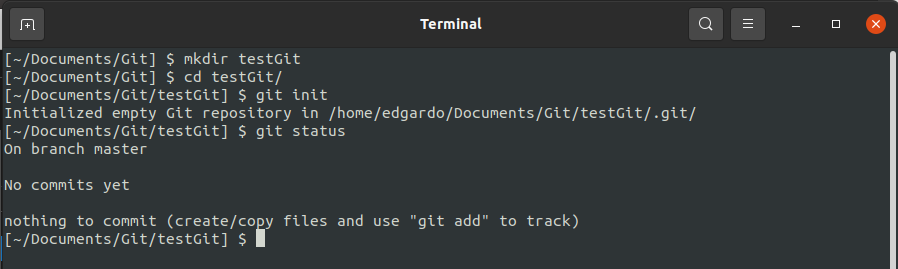
\includegraphics{graphGit_01.png}

    \hypertarget{agregar-un-nuevo-archivo}{%
\subsection{Agregar un nuevo archivo}\label{agregar-un-nuevo-archivo}}

Para añadir un nuevo archivo al control de versiones o para registrar
algún cambio para el siguiente commit, introduce el comando git add y el
nombre de este archivo, que debe encontrarse en tu directorio de
trabajo. En nuestro tutorial, añadiremos un documento de texto llamado
``Test'' como ejemplo:

\begin{quote}
touch Test.txt
\end{quote}

\begin{quote}
\emph{git add Test.txt}
\end{quote}

Después, cuando vuelvas a comprobar el estado del repositorio, verás que
el documento está a la espera de someterse a la siguiente fase de
confirmación de cambios del proyecto, en que estos se aceptarán o no
(\emph{Changes to be commited}):

    \begin{figure}
\centering
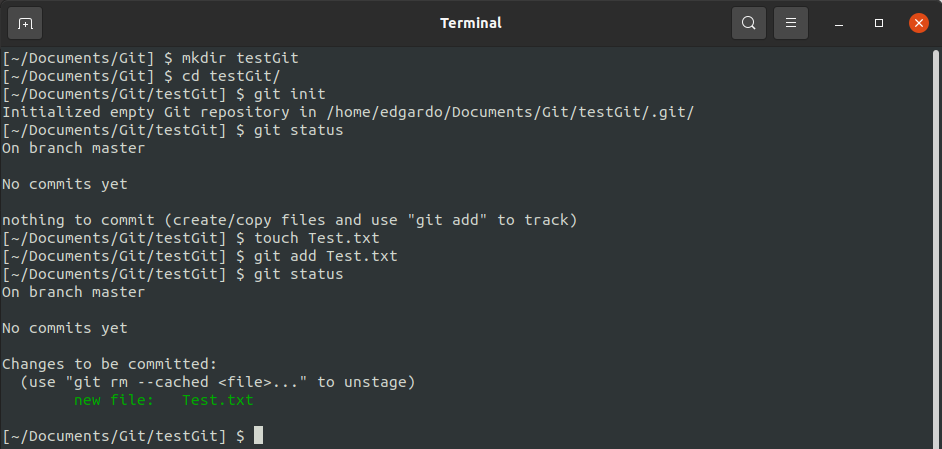
\includegraphics{graphGit_02.png}
\caption{graphGit\_02.png}
\end{figure}

    \hypertarget{confirmar-los-cambios-mediante-commit-y-auxf1adirlos-al-head}{%
\subsection{Confirmar los cambios mediante commit y añadirlos al
HEAD}\label{confirmar-los-cambios-mediante-commit-y-auxf1adirlos-al-head}}

Cualquier cambio que hayas propuesto incorporar al proyecto, como hemos
explicado en el punto anterior, debe confirmarse con commit para que se
incluya en el HEAD. El HEAD es una especie de índice que apunta al
último commit efectuado en el entorno de trabajo Git actual (también
llamado ``rama''). El comando para hacerlo es el siguiente:

\emph{Aqui escribimos una nota, explicando que cambios hicimos, en este
caso decimos que `Hemos agregado el archivo TestGit.txt'}

\begin{quote}
git commit -a -m ``Hemos agregado el archivo TestGit.txt''
\end{quote}

Si no ponemos \texttt{-a\ -m}, luego de ejecutar el comando
\texttt{git\ commit}, Git inicia automáticamente el editor que
configuraste como predeterminado durante la instalación o que el propio
sistema abre por defecto.\\
En el documento, puedes añadir un comentario personal sobre el commit
planificado, en el que las líneas anotadas se separan por punto y coma
y, por lo tanto, no se muestran más adelante.

\begin{quote}
Nota Antes de ejecutar el comando git commit, no te olvides de comprobar
si has marcado todos los cambios que deseas incluir en el repositorio
remoto (con git add). De lo contrario, estos serán ignorados, incluso si
se encuentran en la copia de trabajo guardada en el directorio.
\end{quote}

Luego Git creará el commit y si además hacemos \texttt{git\ status},
veremos lo siguiente:

    \begin{figure}
\centering
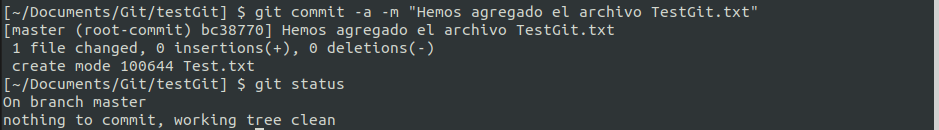
\includegraphics{graphGit_03.png}
\caption{graphGit\_03.png}
\end{figure}

    Como se muestra en la captura de pantalla, después de ejecutar
\texttt{git\ commit}, obtienes un mensaje que resume el commit:\\
1. entre corchetes figuran, por un lado, el nombre de la rama del
proyecto a la que se transfirieron los cambios (en este caso,
\emph{master}, ya que nuestro repositorio de trabajo también es el
repositorio principal),\\
2. por otra parte, la suma de comprobación SHA-1 del commit (en este
caso, bc38770), y\\
3. les siguen el comentario que anotó el propio usuario (aquí, ``Hemos
agregado el archivo TestGit.txt'') y algunos datos concretos sobre los
cambios:\\
\emph{1 file changed, 0 insertions(+), 0 deletions(-)}\\
\emph{create mode 100644 Test.txt}

    \hypertarget{revisar-o-deshacer-commits-ejecutados}{%
\subsection{Revisar o deshacer commits
ejecutados}\label{revisar-o-deshacer-commits-ejecutados}}

Una vez aceptados los cambios mediante el comando commit, puedes editar
el contenido o eliminarlo por completo en cualquier momento más
adelante.\\
Por ejemplo, un caso típico sería precipitarse al ejecutar commit y
olvidarse de algún archivo o configuración importante.\\
En este caso, puedes registrar archivos nuevos o modificados a
posteriori mediante el comando \texttt{git\ add} y volver a
transferirlos.\\
Para ello, añade \texttt{-\/-amend} al comando estándar:

\begin{quote}
\$ git add Test\_02.txt
\end{quote}

\begin{quote}
\$ git commit --amend
\end{quote}

Si quieres deshacer el último commit generado, puedes hacerlo con el
siguiente comando de \texttt{Git}:

\begin{quote}
\$ git reset --soft HEAD\textasciitilde{}1
\end{quote}

Este comando cancela el commit registrado por última vez en el HEAD.\\
Los archivos que contiene se restablecen como ``cambios planificados
para el próximo commit'' en el estado del proyecto.

Si lo que quieres es eliminar por completo los datos introducidos,
ejecuta el siguiente comando en lugar del anterior:

\begin{quote}
\$ git reset --hard HEAD\textasciitilde{}1
\end{quote}

    \hypertarget{mostrar-el-historial-de-commits}{%
\subsection{Mostrar el historial de
commits}\label{mostrar-el-historial-de-commits}}

Aprender a gestionar proyectos con \texttt{Git} es especialmente útil
debido a las características básicas de control de versiones que ofrece
el sistema.\\
Por ejemplo, una gran ventaja de este programa de código abierto es que
siempre puedes visualizar los últimos cambios que se han realizado en el
repositorio. Para ello, puedes utilizar el siguiente comando de
\texttt{Git}:

\begin{quote}
\$ git log
\end{quote}

De manera predeterminada, el comando \texttt{git\ log} enumera los
\emph{commits} generados en orden cronológico inverso:\\
1. la suma de comprobación SHA-1, 2. el autor (nombre y dirección de
correo electrónico) y 3. la fecha de cada commit.

Además, se muestra un comentario individual que sirve a todos los
usuarios como indicador para poder buscar rápidamente las versiones.\\
En un apartado anterior de este tutorial de \texttt{Git}, generamos un
solo commit con el mensaje ````Hemos agregado el archivo
TestGit.txt''''.

Al ejecutar el comando, se nos muestra el archivo solicitado:

    \begin{figure}
\centering
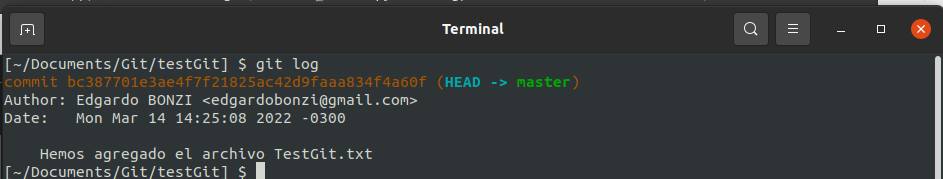
\includegraphics{graphGit_04.png}
\caption{graphGit\_04.png}
\end{figure}

    El comando \texttt{git\ log} también puede modificarse utilizando varios
parámetros.

En la siguiente tabla, te mostramos algunas de las posibilidades:

\begin{longtable}[]{@{}ll@{}}
\toprule
\begin{minipage}[b]{0.21\columnwidth}\raggedright
Parámetros para git log\strut
\end{minipage} & \begin{minipage}[b]{0.73\columnwidth}\raggedright
Descripción\strut
\end{minipage}\tabularnewline
\midrule
\endhead
\begin{minipage}[t]{0.21\columnwidth}\raggedright
-p\strut
\end{minipage} & \begin{minipage}[t]{0.73\columnwidth}\raggedright
Muestra también los cambios incluidos en un commit\strut
\end{minipage}\tabularnewline
\begin{minipage}[t]{0.21\columnwidth}\raggedright
-2\strut
\end{minipage} & \begin{minipage}[t]{0.73\columnwidth}\raggedright
Enumera solo los dos últimos commits ejecutados\strut
\end{minipage}\tabularnewline
\begin{minipage}[t]{0.21\columnwidth}\raggedright
--stat\strut
\end{minipage} & \begin{minipage}[t]{0.73\columnwidth}\raggedright
Añade una pequeña estadística a cada registro que muestra qué archivos
se han\strut
\end{minipage}\tabularnewline
\begin{minipage}[t]{0.21\columnwidth}\raggedright
\strut
\end{minipage} & \begin{minipage}[t]{0.73\columnwidth}\raggedright
modificado y cuántas líneas se han insertado o eliminado\strut
\end{minipage}\tabularnewline
\begin{minipage}[t]{0.21\columnwidth}\raggedright
--pretty\strut
\end{minipage} & \begin{minipage}[t]{0.73\columnwidth}\raggedright
Cambia el formato de salida con diferentes posibilidades;\strut
\end{minipage}\tabularnewline
\begin{minipage}[t]{0.21\columnwidth}\raggedright
--abbrev-commit\strut
\end{minipage} & \begin{minipage}[t]{0.73\columnwidth}\raggedright
Muestra solo los primeros caracteres de una suma de comprobación
\texttt{SHA-1}\strut
\end{minipage}\tabularnewline
\begin{minipage}[t]{0.21\columnwidth}\raggedright
--relative-date\strut
\end{minipage} & \begin{minipage}[t]{0.73\columnwidth}\raggedright
Muestra la fecha de un cambio en formato relativo (por ejemplo, ``hace
dos semanas'')\strut
\end{minipage}\tabularnewline
\bottomrule
\end{longtable}

    \hypertarget{como-configurar-la-key}{%
\subsection{Como configurar la key}\label{como-configurar-la-key}}

\$ git config --global credential.helper store --file
\textasciitilde{}/.ssh/git\_rsa.pub

    \begin{tcolorbox}[breakable, size=fbox, boxrule=1pt, pad at break*=1mm,colback=cellbackground, colframe=cellborder]
\prompt{In}{incolor}{ }{\boxspacing}
\begin{Verbatim}[commandchars=\\\{\}]

\end{Verbatim}
\end{tcolorbox}


To be continue ...
    % Add a bibliography block to the postdoc
    
    
    
\end{document}
